% Slides for 2024-05-13
% To create a slide, use the following:
% \begin{frame}{TITLE}
%     BODY
% \end{frame}

% To create a slide with a bullet list, use the following:
% \begin{frame}{TITLE}
%     \begin{itemize}
%         \item ITEM 1
%         \item ITEM 2
%     \end{itemize}    
% \end{frame}

% To create a slide with numbered list, use the following:
% \begin{frame}{TITLE}
%     \begin{enumerate}
%         \item ITEM 1
%         \item ITEM 2
%     \end{enumerate}
% \end{frame}

% To create a slide with a graphic:
% 1. Add the graphic to this folder (named picture.png)
% 2. Use the following:
% \begin{frame}{TITLE}
%     \centering
%     \includegraphics[height=0.7\textheight,width=0.7\textwidth,keepaspectratio]{picture.png}
% \end{frame}

% To create a slide with two columns, use the following:
% \begin{frame}{TITLE}
%     \begin{columns}
%         \begin{column}{0.5\textwidth}
%             COLUMN 1 BODY
%         \end{column}
%         \begin{column}{0.5\textwidth}
%             COLUMN 2 BODY
%         \end{column}
%     \end{columns}
% \end{frame}


\begin{frame}{How do we verify model performance?}
    \begin{itemize}
        \item "When is model useful for Collaborators"
        \item Interested more in FP than FN
        \item select higher confidence in practice
        \item GOAL: Verify high confidence clips
        \item Following method allowed for labeling
        \item Verified 522 clips, 119 species
    \end{itemize}
\end{frame}

\begin{frame}{Verify the top X (ex: 1) clips}
    \centering
    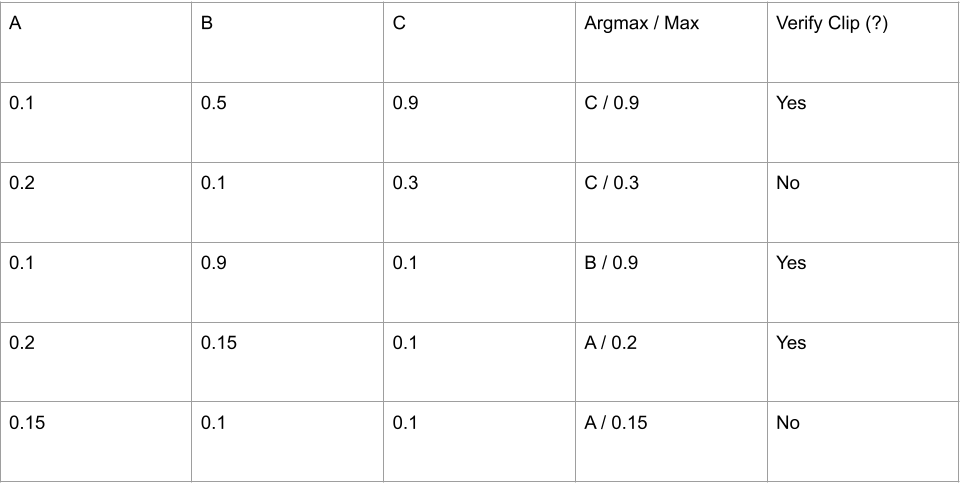
\includegraphics[height=0.7\textheight,width=0.7\textwidth,keepaspectratio]{./images/clip_selection_process.png}
\end{frame}

\begin{frame}{"Confidence chart"}

    \centering
    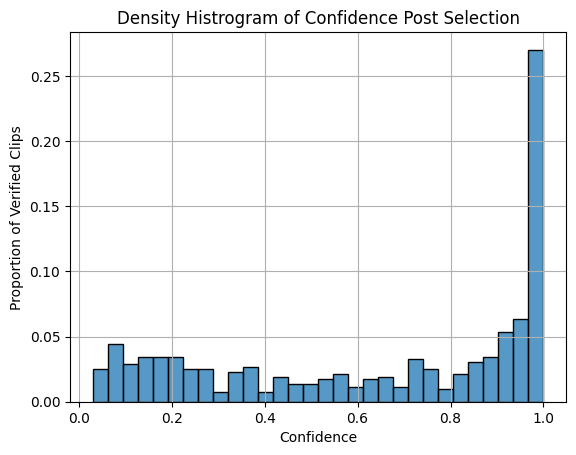
\includegraphics[height=0.7\textheight,width=0.7\textwidth,keepaspectratio]{./images/prop_confidence.png}

\end{frame}

\begin{frame}{"Confidence chart"}

    \centering
    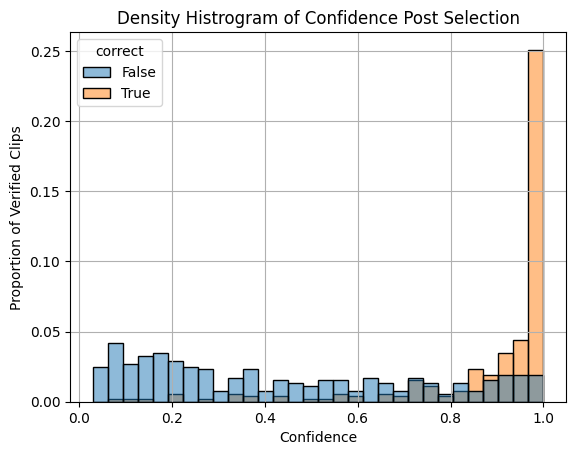
\includegraphics[height=0.7\textheight,width=0.7\textwidth,keepaspectratio]{./images/prop_confidence_facet.png}

\end{frame}

\begin{frame}{"ROC"}

    \centering
    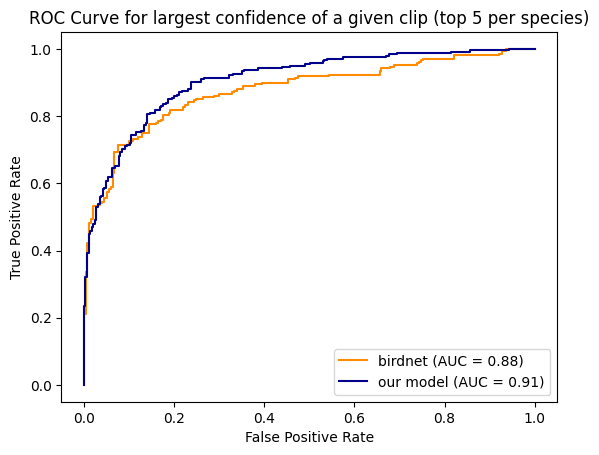
\includegraphics[height=0.7\textheight,width=0.7\textwidth,keepaspectratio]{./images/roc.png}

\end{frame}

\begin{frame}{Discussion}
    \begin{itemize}
        \item Doesn't account for secondary birds
        \item Verifcation took about 6-8 hours
        \item Concern with not random sampling
        \item I am not an Ornithologist
        \item Models can be useful!
    \end{itemize}
\end{frame}

\begin{frame}{Template Matching Motivation}
    \begin{itemize}
        \item Big picture: one call/day
        \item 1000 species to look at
        \item Which ones exist in data?
    \end{itemize}
\end{frame}

\begin{frame}{Template Matching}
    So far:
    \begin{itemize}
        \item Piha: 0.59 precision
        \item Attila: running
    \end{itemize}
    Plan:
    \begin{itemize}
        \item Get human-verified tm results
        \item Train Efficientnet, trained on XC
        \item Compare results to Jacob's baseline
    \end{itemize}
\end{frame}